\chapter{Resultados e Discussões} \label{cap::resultados}

Os resultados das simulações de cada tarefa proposta são apresentados nas
seções~\ref{sec::resultados_t1} e \ref{sec::resultados_t2} para os seguintes
casos de base:
%
\begin{enumerate*}[label=\emph{\roman*})]
	\item base rígida;
	\item base de testes;
	\item base modular PRP;
	\item base telescópica PRPP.
\end{enumerate*}
%

Em todos os casos são avaliados os erros de posicionamento, velocidade e
orientação da ferramenta, ao longo de toda a tarefa. Na
seção~\ref{sec::comparacao} são comparados os resultados das tarefas para as
diferentes bases.

% -.~.-.~.-.~.-.~.-.~.-.~.-.~.-.~.-.~.-.~.-.~.-
\section{Resultados de simulação da Tarefa 1} \label{sec::resultados_t1}


\subsection{Base rígida -- Tarefa 1} \label{sec::res_rigida}

Seguem os resultados do modelo de base rígida que utiliza o modelo MBS --
Robô.
A Figura~\ref{fig::t1_anima3D_base_rig} apresenta o resultado da simulação no ambiente
3D para a Tarefa 1.

\begin{figure}[h!]
	\centering 
 	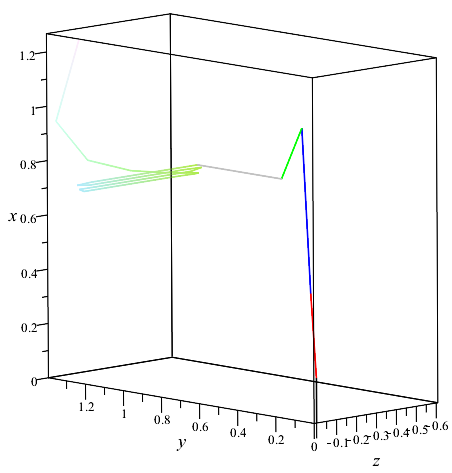
\includegraphics[width=0.50\textwidth]{figs/t1_anima3D_base_rig}
 	\caption{Simulação no ambiente 3D para a Tarefa 1}
 	\label{fig::t1_anima3D_base_rig}
\end{figure}

Estes resultados representam uma referência para posterior comparação com os
resultados obtidos para o modelo MBS acoplado.

\subsubsection{Posição da ferramenta}

Os resultados de simulação da posição da ponta da ferramenta para Tarefa 1 são
apresentados a seguir. A Figura~\ref{fig::t1_posf_base_rig} fornece o valor de
cada coordenada $x, y, z$ no referencial inercial (linha cheia) e também o valor
de referência (linha tracejada), fornecido pela cinemática inversa. A
Figura~\ref{fig::t1_erroposf_base_rig} fornece o erro de posição, ou seja, a
diferença entre o valor de referência dado pela cinemática inversa e o efetivo,
de cada coordenada, assim como o erro absoluto (linha tracejada).

\begin{figure}[h!]
	\centering 
 	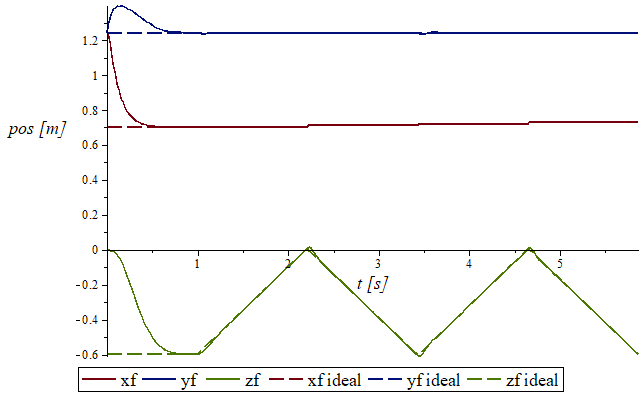
\includegraphics[width=0.75\textwidth]{figs/t1_posf_base_rig}
 	\caption{Posições das coordenadas da ferramenta para base rígida -- Tarefa 1}
 	\label{fig::t1_posf_base_rig}
\end{figure}

\begin{figure}[h!]
	\centering 
 	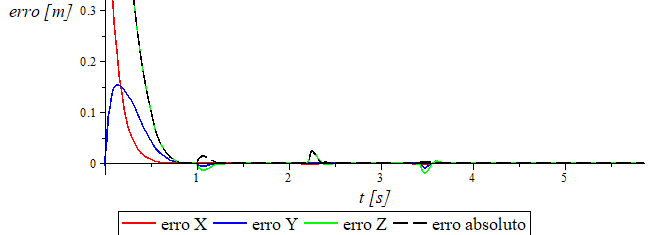
\includegraphics[width=0.75\textwidth]{figs/t1_erroposf_base_rig}
 	\caption{Erro de posição da ferramenta para base rígida -- Tarefa 1}
 	\label{fig::t1_erroposf_base_rig}
\end{figure}


\subsubsection{Velocidade da ferramenta}

São apresentados os gráficos da velocidade da ponta da ferramenta (linhas
cheias) e as velocidades de referência dadas pela cinemática inversa (linhas
tracejadas), na Figura~\ref{fig::t1_velf_base_rig}. Na
Figura~\ref{fig::t1_errovelf_base_rig} os erros em relação a velocidade de
referência, no referencial inercial.

\begin{figure}[h!]
	\centering 
 	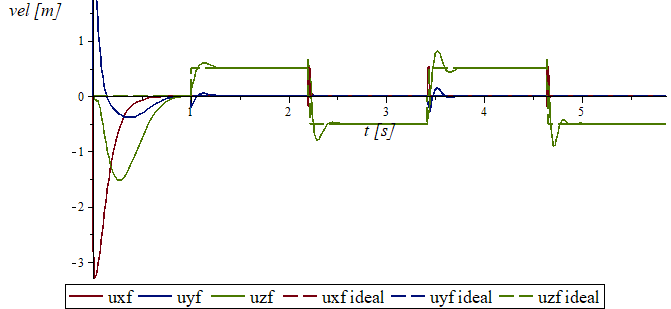
\includegraphics[width=0.75\textwidth]{figs/t1_velf_base_rig}
 	\caption{Velocidades das coordenadas da ferramenta para base rígida -- Tarefa 1}
 	\label{fig::t1_velf_base_rig}
\end{figure}

\begin{figure}[h!]
	\centering 
 	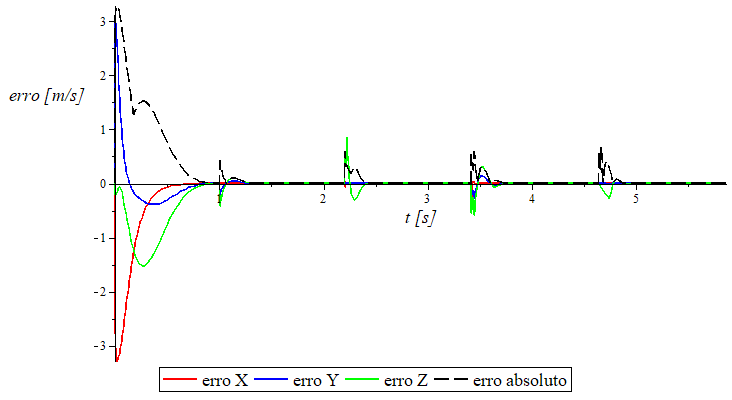
\includegraphics[width=0.75\textwidth]{figs/t1_errovelf_base_rig}
 	\caption{Erro de velocidade da ferramenta para base rígida --
 	Tarefa 1}
 	\label{fig::t1_errovelf_base_rig}
\end{figure}


\subsubsection{Orientação da ferramenta}

O erro de orientação da ferramenta é resultado da matriz de rotação entre o
referencial inercial e a orientação do pulso do robô, em função dos ângulos de
Euler, para a orientação desejada. Faz-se uma transformação da matriz de rotação
em eixo e ângulo, de acordo com as equações~\ref{eq::ang_erro} e
\ref{eq::eixo_erro}. A Figura~\ref{fig::t1_erroori_base_rig} apresenta o
erro de orientação, representado pelo ângulo $\theta$, para a Tarefa 1.

\begin{figure}[h!]
	\centering 
 	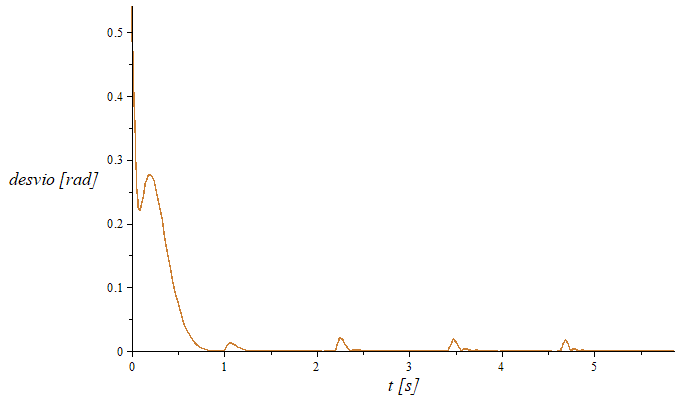
\includegraphics[width=0.75\textwidth]{figs/t1_erroori_base_rig}
 	\caption{Erro de orientação da ferramenta para base rígida -- Tarefa
 	1}
 	\label{fig::t1_erroori_base_rig}
\end{figure}



\subsection{Base de testes -- Tarefa 1} \label{sec::res_testes}

Apresenta-se os resultados das trajetórias considerando o manipulador montado
sobre a base de testes, da seção~\ref{sec::base_testes}, realizando a Tarefa 1.

\subsubsection{Posição do ponto virtual}

O reusltado da Figura~\ref{fig::t1_q123456_base_testes} apresenta a variação das
coordenadas generalizadas $q1$ a $q3$, referentes às translações, e $q4$ a $q6$,
referentes às rotações do ponto virtual de acoplamento base e robô. A
Figura~\ref{fig::t1_pvirtural_base_testes} ilustra o rastro da posição do ponto
virtual (origem do robô) no ambiente 3D.

\begin{figure}[h]
    \centering
    \begin{subfigure}[b]{0.45\textwidth}
        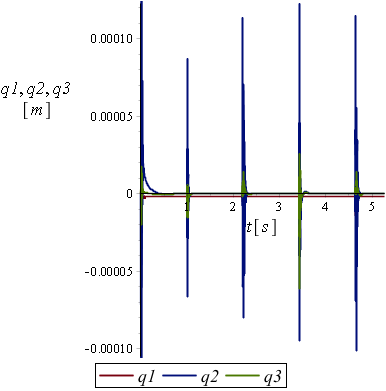
\includegraphics[width=\textwidth]{figs/t1_q123_base_testes}
        \caption{Deslocamentos do ponto virtual}
        \label{fig::t1_q123_base_testes}
    \end{subfigure}
    \quad %add desired spacing between images, e. g. ~, \quad, \qquad, \hfill
    % etc.
      %(or a blank line to force the subfigure onto a new line)
    \begin{subfigure}[b]{0.45\textwidth}
        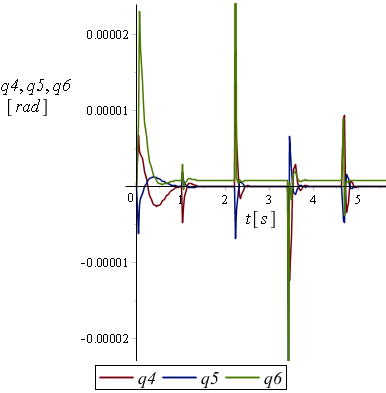
\includegraphics[width=\textwidth]{figs/t1_q456_base_testes}
        \caption{Rotações do ponto virtual}
        \label{fig::t1_q456_base_testes}
    \end{subfigure}
    \caption{Variações de posição e orientação da base de testes -- Tarefa 1}
    \label{fig::t1_q123456_base_testes}
\end{figure}

\begin{figure}[h!]
	\centering 
 	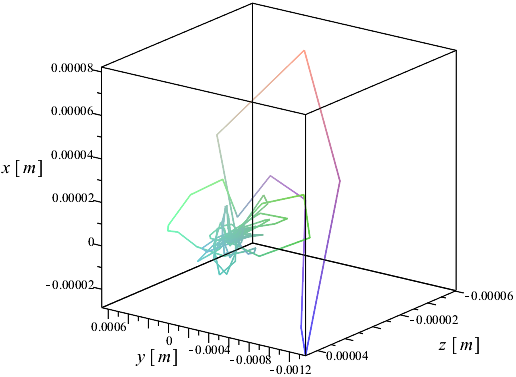
\includegraphics[width=0.70\textwidth]{figs/t1_pvirtural_base_testes}
 	\caption{Rastro da posição do ponto virtual da base de testes -- Tarefa 1}
 	\label{fig::t1_pvirtural_base_testes}
\end{figure}


\subsubsection{Posição da ferramenta}

A Figura~\ref{fig::t1_posf_base_testes} fornece as posições efetiva (linhas
cheias) e ideal (linhas tracejadas). E a
Figura~\ref{fig::t1_erroposf_base_testes} o erro de cada coordenada, com
respeito ao referencial inercial.

\begin{figure}[h!]
	\centering 
 	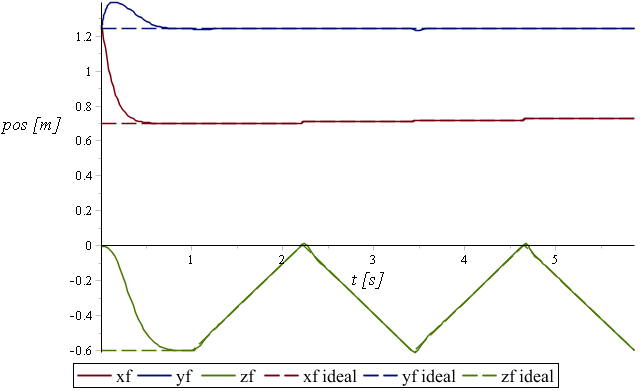
\includegraphics[width=0.75\textwidth]{figs/t1_posf_base_testes}
 	\caption{Posições das coordenadas da ferramenta para base de testes -- Tarefa
 	1}
 	\label{fig::t1_posf_base_testes}
\end{figure}

\begin{figure}[h!]
	\centering 
 	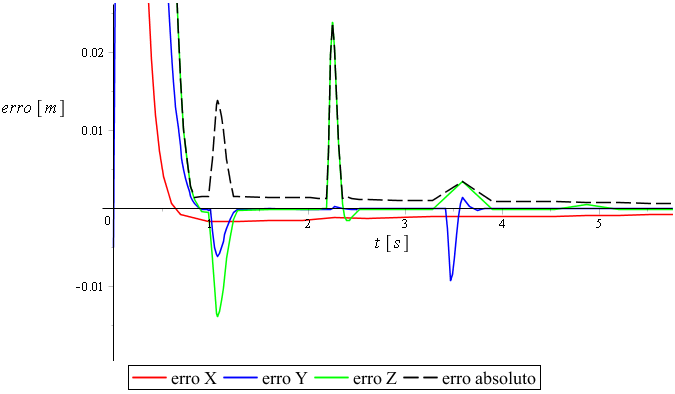
\includegraphics[width=0.75\textwidth]{figs/t1_erroposf_base_testes}
 	\caption{Erro de posição da ferramenta para base de testes -- Tarefa 1}
 	\label{fig::t1_erroposf_base_testes}
\end{figure}



\subsubsection{Velocidade da ferramenta}

São apresentados os gráficos da velocidade da ponta da ferramenta (linhas
cheias) e as velocidades de referência dadas pela cinemática inversa (linhas
tracejadas), na Figura~\ref{fig::t1_velf_base_testes} e na
Figura~\ref{fig::t1_errovelf_base_testes} os erros em relação a velocidade de
referência, no referencial inercial.

\begin{figure}[h!]
	\centering 
 	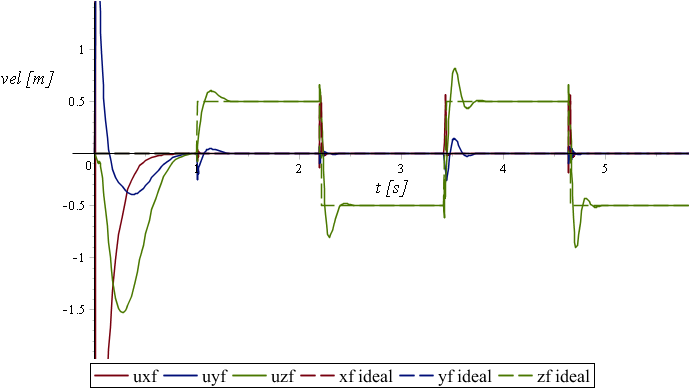
\includegraphics[width=0.75\textwidth]{figs/t1_velf_base_testes}
 	\caption{Velocidades das coordenadas da ferramenta base de testes --
 	Tarefa 1}
 	\label{fig::t1_velf_base_testes}
\end{figure}

\begin{figure}[h!]
	\centering 
 	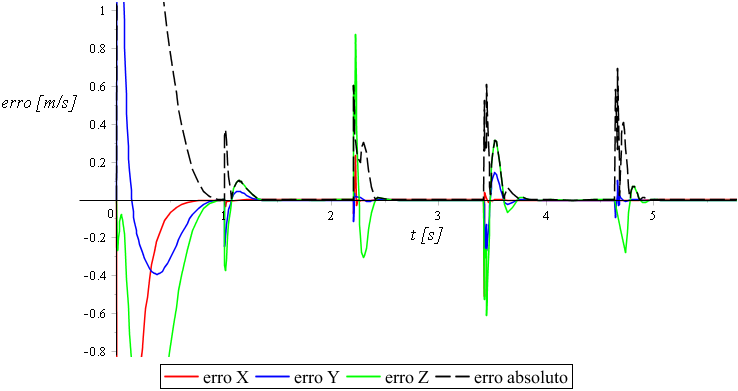
\includegraphics[width=0.75\textwidth]{figs/t1_errovelf_base_testes}
 	\caption{Erro de velocidade da ferramenta para base de testes --
 	Tarefa 1}
 	\label{fig::t1_errovelf_base_testes}
\end{figure}


\subsubsection{Orientação da ferramenta}

A Figura~\ref{fig::t1_erroori_base_testes} apresenta o erro de orientação,
representado pelo ângulo $\theta$.

\begin{figure}[h!]
	\centering 
 	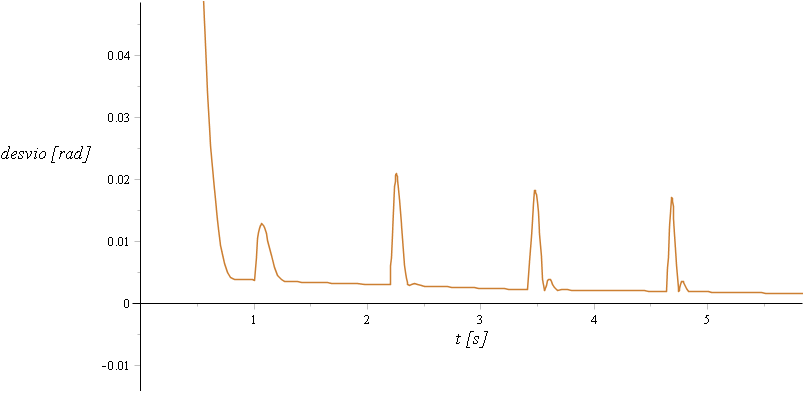
\includegraphics[width=0.75\textwidth]{figs/t1_erroori_base_testes}
 	\caption{Erro de orientação da ferramenta para base de testes -- Tarefa
 	1}
 	\label{fig::t1_erroori_base_testes}
\end{figure}

\clearpage
\subsection{Base modular PRP -- Tarefa 1} \label{sec::res_prp}

Apresenta-se os resultados das trajetórias considerando o manipulador montado
sobre a base modular PRP, da seção~\ref{sec::base_prp}, realizando a Tarefa 1.

\subsubsection{Posição do ponto virtual}

O reusltado da Figura~\ref{fig::t1_q123456_base_prp} apresenta a variação das
coordenadas generalizadas $q1$ a $q3$, referentes às translações, e $q4$ a $q6$,
referentes às rotações do ponto virtual de acoplamento base e robô. A
Figura~\ref{fig::t1_pvirtural_base_prp} ilustra o rastro da posição do ponto
virtual (origem do robô) no ambiente 3D.

\begin{figure}[h]
    \centering
    \begin{subfigure}[b]{0.48\textwidth}
        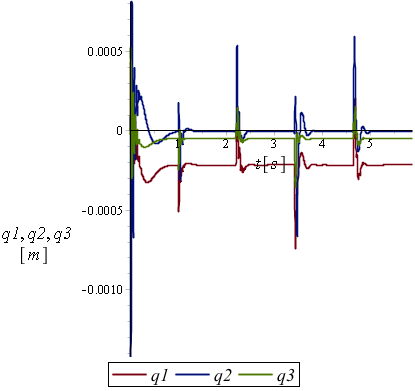
\includegraphics[width=\textwidth]{figs/t1_q123_base_prp}
        \caption{Deslocamentos do ponto virtual}
        \label{fig::t1_q123_base_prp}
    \end{subfigure}
    \quad %add desired spacing between images, e. g. ~, \quad, \qquad, \hfill
    % etc.
      %(or a blank line to force the subfigure onto a new line)
    \begin{subfigure}[b]{0.48\textwidth}
        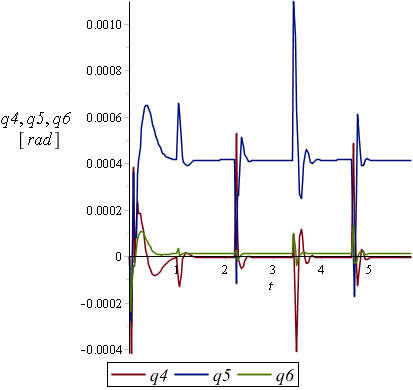
\includegraphics[width=\textwidth]{figs/t1_q456_base_prp}
        \caption{Rotações do ponto virtual}
        \label{fig::t1_q456_base_prp}
    \end{subfigure}
    \caption{Variações de posição e orientação da base PRP -- Tarefa 1}
    \label{fig::t1_q123456_base_prp}
\end{figure}

\begin{figure}[h!]
	\centering 
 	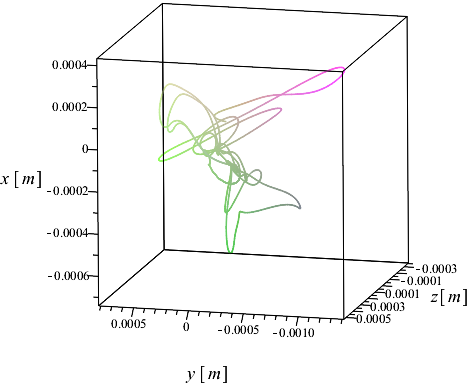
\includegraphics[width=0.70\textwidth]{figs/t1_pvirtural_base_prp}
 	\caption{Rastro da posição do ponto virtual da base PRP-- Tarefa 1}
 	\label{fig::t1_pvirtural_base_prp}
\end{figure}


\subsubsection{Posição da ferramenta}

A Figura~\ref{fig::t1_posf_base_prp} fornece as posições efetiva (linhas cheias)
e ideal (linhas tracejadas). E a Figura~\ref{fig::t1_erroposf_base_prp} o erro
de cada coordenada, com respeito ao referencial inercial.

\begin{figure}[h!]
	\centering 
 	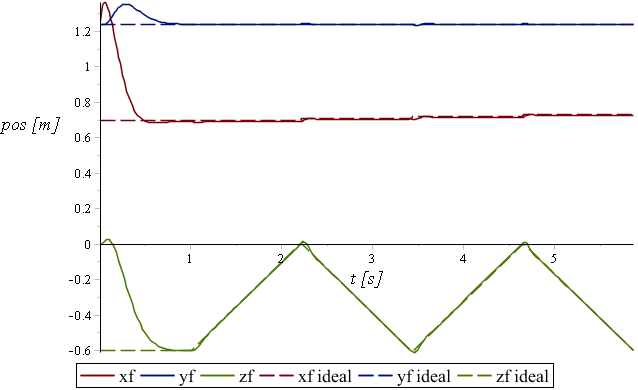
\includegraphics[width=0.75\textwidth]{figs/t1_posf_base_prp}
 	\caption{Posições das coordenadas da ferramenta para base PRP -- Tarefa
 	1}
 	\label{fig::t1_posf_base_prp}
\end{figure}

\begin{figure}[h!]
	\centering 
 	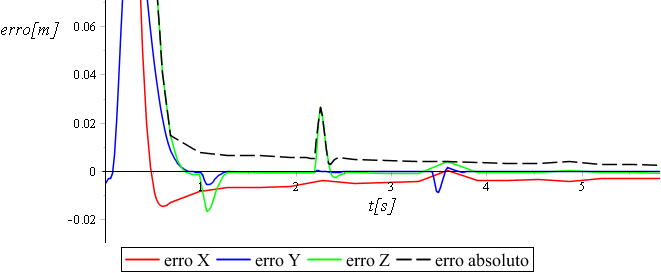
\includegraphics[width=0.75\textwidth]{figs/t1_erroposf_base_prp}
 	\caption{Erro de posição da ferramenta para base PRP -- Tarefa 1}
 	\label{fig::t1_erroposf_base_prp}
\end{figure}



\subsubsection{Velocidade da ferramenta}

São apresentados os gráficos da velocidade da ponta da ferramenta (linhas
cheias) e as velocidades de referência dadas pela cinemática inversa (linhas
tracejadas), na Figura~\ref{fig::t1_velf_base_prp} e na
Figura~\ref{fig::t1_errovelf_base_prp} os erros em relação a velocidade de
referência, no referencial inercial.

\begin{figure}[h!]
	\centering 
 	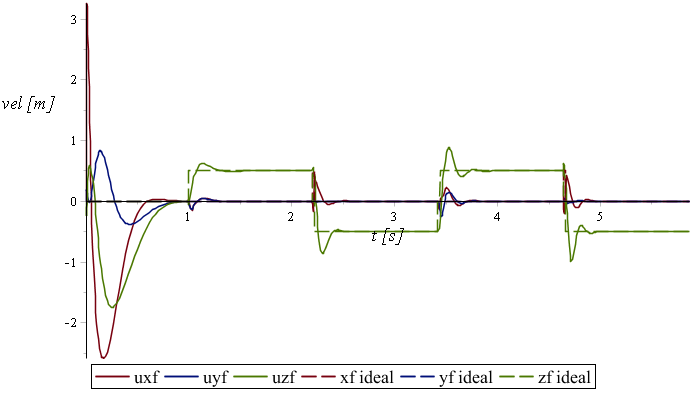
\includegraphics[width=0.75\textwidth]{figs/t1_velf_base_prp}
 	\caption{Velocidades das coordenadas da ferramenta base PRP --
 	Tarefa 1}
 	\label{fig::t1_velf_base_prp}
\end{figure}

\begin{figure}[h!]
	\centering 
 	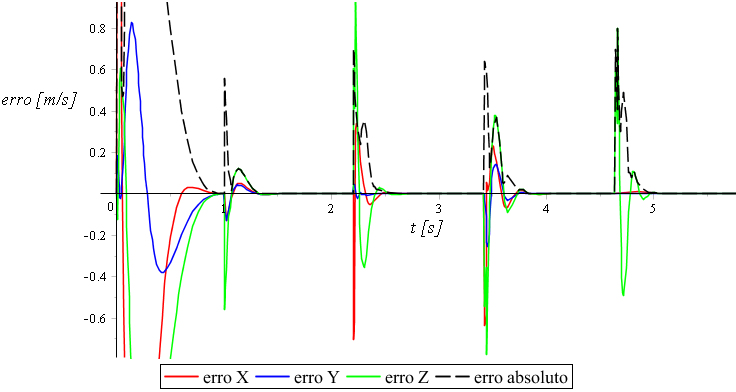
\includegraphics[width=0.75\textwidth]{figs/t1_errovelf_base_prp}
 	\caption{Erro de velocidade da ferramenta para base PRP --
 	Tarefa 1}
 	\label{fig::t1_errovelf_base_prp}
\end{figure}


\subsubsection{Orientação da ferramenta}

A Figura~\ref{fig::t1_erroori_base_prp} apresenta o erro de orientação,
representado pelo ângulo $\theta$.

\begin{figure}[h!]
	\centering 
 	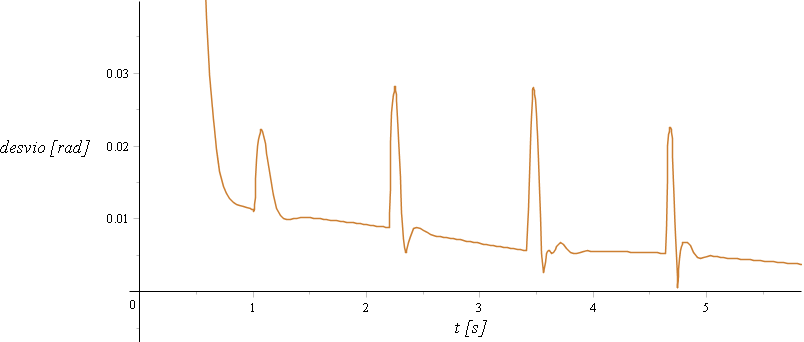
\includegraphics[width=0.75\textwidth]{figs/t1_erroori_base_prp}
 	\caption{Erro de orientação da ferramenta para base PRP -- Tarefa
 	1}
 	\label{fig::t1_erroori_base_prp}
\end{figure}


\clearpage
\subsection{Base telescópica PRPP -- Tarefa 1} \label{sec::res_prpp}

Apresenta-se os resultados das trajetórias considerando o manipulador montado
sobre a base modular PRP, da seção~\ref{sec::base_prpp}, realizando a Tarefa 1.

\subsubsection{Posição do ponto virtual}

O reusltado da Figura~\ref{fig::t1_q123456_base_prpp} apresenta a variação das
coordenadas generalizadas $q1$ a $q3$, referentes às translações, e $q4$ a $q6$,
referentes às rotações do ponto virtual de acoplamento base e robô. A
Figura~\ref{fig::t1_pvirtural_base_prpp} ilustra o rastro da posição do ponto
virtual (origem do robô) no ambiente 3D.

\begin{figure}[h]
    \centering
    \begin{subfigure}[b]{0.48\textwidth}
        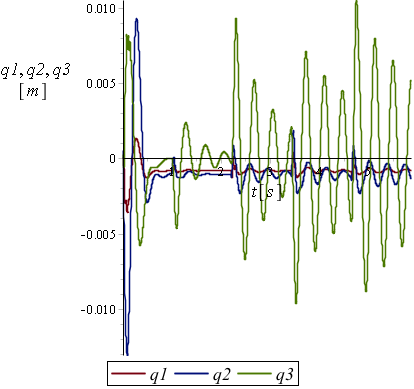
\includegraphics[width=\textwidth]{figs/t1_q123_base_prpp}
        \caption{Deslocamentos do ponto virtual}
        \label{fig::t1_q123_base_prpp}
    \end{subfigure}
    \quad %add desired spacing between images, e. g. ~, \quad, \qquad, \hfill
    % etc.
      %(or a blank line to force the subfigure onto a new line)
    \begin{subfigure}[b]{0.48\textwidth}
        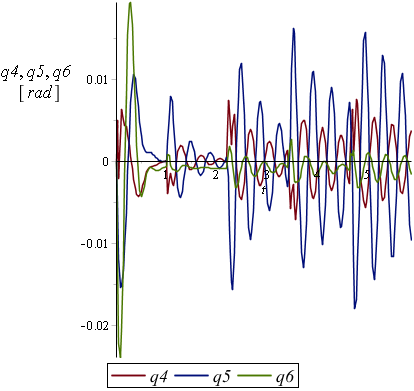
\includegraphics[width=\textwidth]{figs/t1_q456_base_prpp}
        \caption{Rotações do ponto virtual}
        \label{fig::t1_q456_base_prpp}
    \end{subfigure}
    \caption{Variações de posição e orientação da base PRPP -- Tarefa 1}
    \label{fig::t1_q123456_base_prpp}
\end{figure}

\begin{figure}[h!]
	\centering 
 	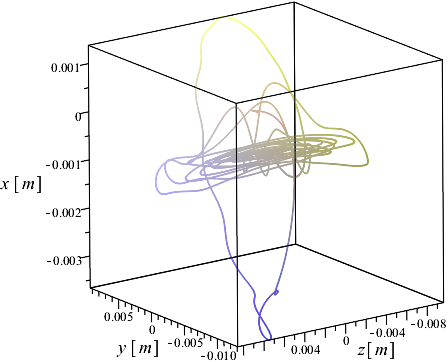
\includegraphics[width=0.65\textwidth]{figs/t1_pvirtural_base_prpp}
 	\caption{Rastro da posição do ponto virtual da base PRPP -- Tarefa 1}
 	\label{fig::t1_pvirtural_base_prpp}
\end{figure}


\subsubsection{Posição da ferramenta}

A Figura~\ref{fig::t1_posf_base_prpp} fornece as posições efetiva (linhas cheias)
e ideal (linhas tracejadas). E a Figura~\ref{fig::t1_erroposf_base_prpp} o erro
de cada coordenada, com respeito ao referencial inercial.

\begin{figure}[h!]
	\centering 
 	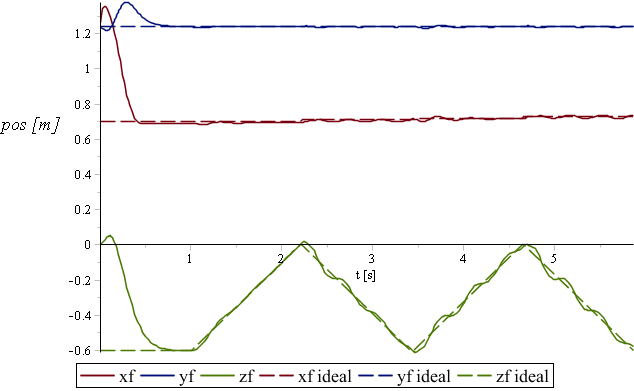
\includegraphics[width=0.75\textwidth]{figs/t1_posf_base_prpp}
 	\caption{Posições das coordenadas da ferramenta para base PRPP -- Tarefa
 	1}
 	\label{fig::t1_posf_base_prpp}
\end{figure}

\begin{figure}[h!]
	\centering 
 	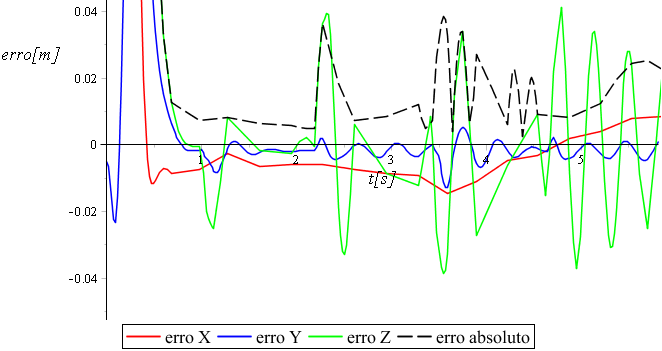
\includegraphics[width=0.75\textwidth]{figs/t1_erroposf_base_prpp}
 	\caption{Erro de posição da ferramenta para base PRPP -- Tarefa 1}
 	\label{fig::t1_erroposf_base_prpp}
\end{figure}

\subsubsection{Velocidade da ferramenta}

São apresentados os gráficos da velocidade da ponta da ferramenta (linhas
cheias) e as velocidades de referência dadas pela cinemática inversa (linhas
tracejadas), na Figura~\ref{fig::t1_velf_base_prpp} e na
Figura~\ref{fig::t1_errovelf_base_prpp} os erros em relação a velocidade de
referência, no referencial inercial.

\begin{figure}[h!]
	\centering 
 	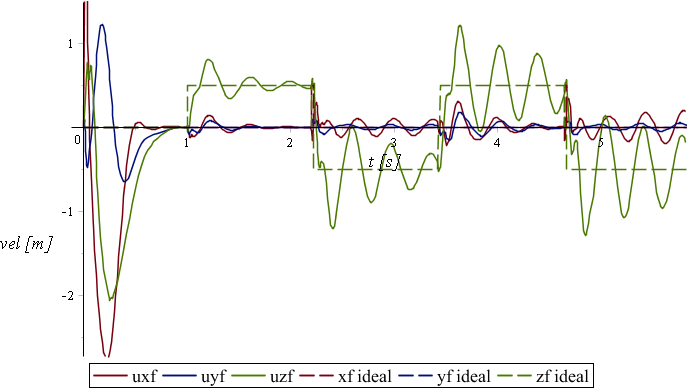
\includegraphics[width=0.75\textwidth]{figs/t1_velf_base_prpp}
 	\caption{Velocidades das coordenadas da ferramenta base PRPP --
 	Tarefa 1}
 	\label{fig::t1_velf_base_prpp}
\end{figure}

\begin{figure}[h!]
	\centering 
 	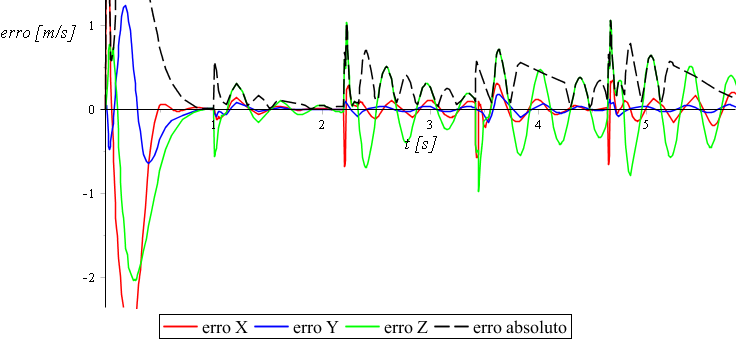
\includegraphics[width=0.75\textwidth]{figs/t1_errovelf_base_prpp}
 	\caption{Erro de velocidade da ferramenta para base PRPP --
 	Tarefa 1}
 	\label{fig::t1_errovelf_base_prpp}
\end{figure}

\subsubsection{Orientação da ferramenta}

A Figura~\ref{fig::t1_erroori_base_prpp} apresenta o erro de orientação,
representado pelo ângulo $\theta$.

\begin{figure}[h!]
	\centering 
 	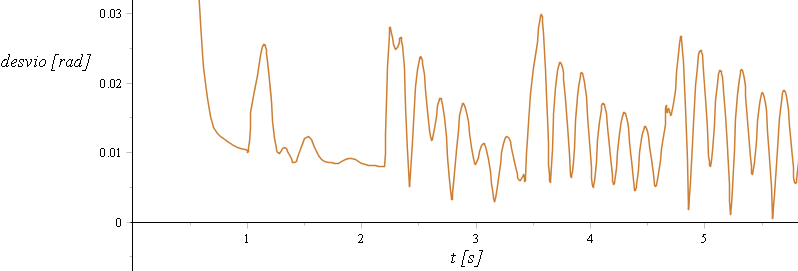
\includegraphics[width=0.75\textwidth]{figs/t1_erroori_base_prpp}
 	\caption{Erro de orientação da ferramenta para base PRPP -- Tarefa
 	1}
 	\label{fig::t1_erroori_base_prpp}
\end{figure}



% -.~.-.~.-.~.-.~.-.~.-.~.-.~.-.~.-.~ TAREFA 2 ~.-.~.-.~.-.~.-.~.-.~.-.~.
\clearpage
\section{Resultados de simulação da Tarefa 2} \label{sec::resultados_t2}

\subsection{Base rígida -- Tarefa 2}

Seguem os resultados do modelo de base rígida que utiliza o modelo MBS --
Robô.
A Figura~\ref{fig::t2_anima3D_base_rig} apresenta o resultado da simulação no ambiente
3D para a Tarefa 2.

\begin{figure}[h!]
	\centering 
 	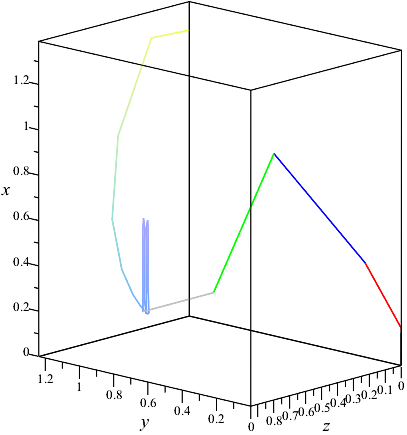
\includegraphics[width=0.50\textwidth]{figs/t2_anima3D_base_rig}
 	\caption{Simulação no ambiente 3D para a Tarefa 2}
 	\label{fig::t2_anima3D_base_rig}
\end{figure}


\subsubsection{Posição da ferramenta}

A Figura~\ref{fig::t2_posf_base_rig} fornece as posições efetiva (linhas cheias)
e ideal (linhas tracejadas). 

\begin{figure}[h!]
	\centering 
 	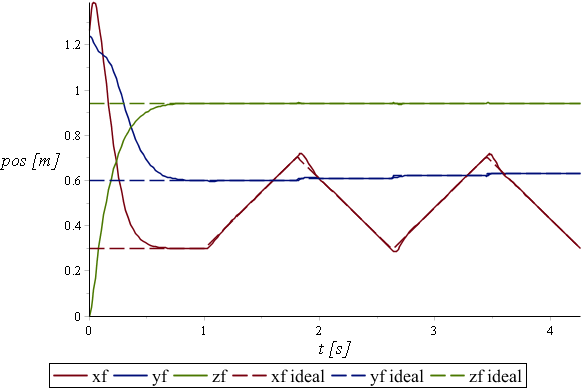
\includegraphics[width=0.75\textwidth]{figs/t2_posf_base_rig}
 	\caption{Posições das coordenadas da ferramenta para base rígida -- Tarefa 2}
 	\label{fig::t2_posf_base_rig}
\end{figure}

E a Figura~\ref{fig::t2_erroposf_base_rig} o erro
de cada coordenada, com respeito ao referencial inercial.

\begin{figure}[h!]
	\centering 
 	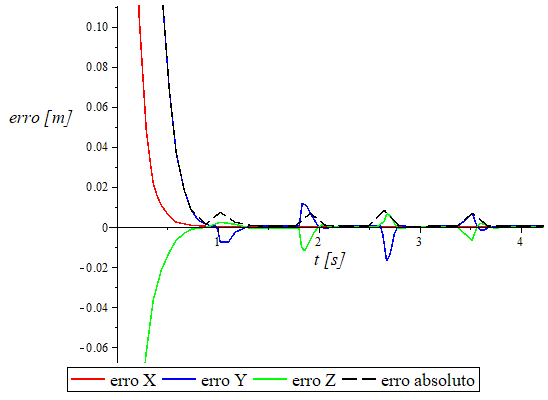
\includegraphics[width=0.75\textwidth]{figs/t2_erroposf_base_rig}
 	\caption{Erro de posição da ferramenta para base rígida -- Tarefa 2}
 	\label{fig::t2_erroposf_base_rig}
\end{figure}


\subsubsection{Velocidade da ferramenta}

São apresentados os gráficos da velocidade da ponta da ferramenta (linhas
cheias) e as velocidades de referência dadas pela cinemática inversa (linhas
tracejadas), na Figura~\ref{fig::t2_velf_base_rig} e na
Figura~\ref{fig::t2_errovelf_base_rig} os erros em relação a velocidade de
referência, no referencial inercial.

\begin{figure}[h!]
	\centering 
 	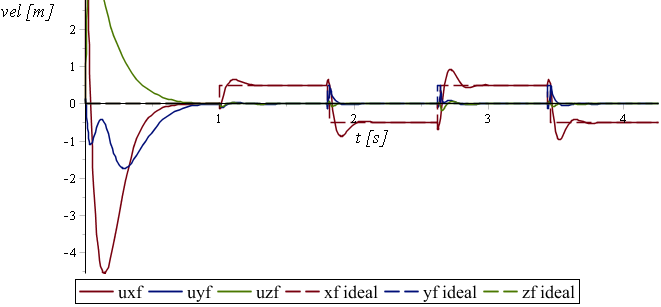
\includegraphics[width=0.75\textwidth]{figs/t2_velf_base_rig}
 	\caption{Velocidades das coordenadas da ferramenta base rígida -- Tarefa
 	2}
 	\label{fig::t2_velf_base_rig}
\end{figure}

\begin{figure}[h!]
	\centering 
 	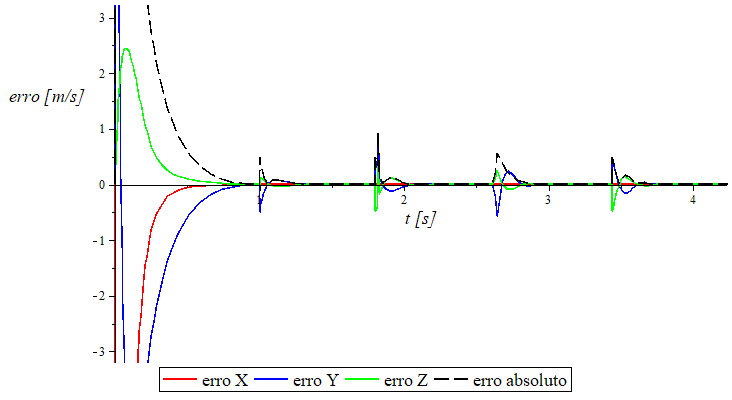
\includegraphics[width=0.75\textwidth]{figs/t2_errovelf_base_rig}
 	\caption{Erro de velocidade da ferramenta para base rígida -- Tarefa 2}
 	\label{fig::t2_errovelf_base_rig}
\end{figure}


\subsubsection{Orientação da ferramenta}

A Figura~\ref{fig::t2_erroori_base_rig} apresenta o erro de orientação da
ferramenta, representado pelo ângulo $\theta$.

\begin{figure}[h!]
	\centering 
 	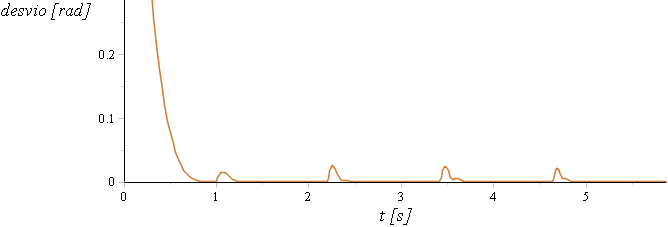
\includegraphics[width=0.75\textwidth]{figs/t2_erroori_base_rig}
 	\caption{Erro de orientação da ferramenta para base rígida -- Tarefa
 	2}
 	\label{fig::t2_erroori_base_rig}
\end{figure}


\subsection{Base de testes -- Tarefa 2}

\subsubsection{Posição do ponto virtual}

O reusltado da Figura~\ref{fig::t2_q123456_base_testes} apresenta a variação das
coordenadas generalizadas $q1$ a $q3$, referentes às translações, e $q4$ a $q6$,
referentes às rotações do ponto virtual de acoplamento base e robô. A
Figura~\ref{fig::t2_pvirtural_base_testes} ilustra o rastro da posição do ponto
virtual (origem do robô) no ambiente 3D.

\begin{figure}[h]
    \centering
    \begin{subfigure}[b]{0.48\textwidth}
        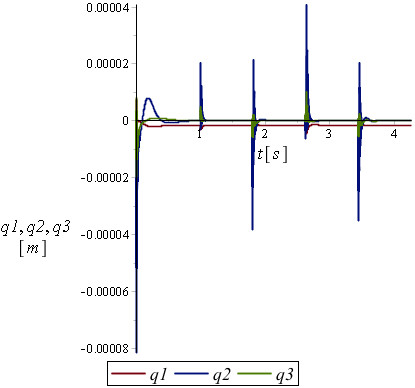
\includegraphics[width=\textwidth]{figs/t2_q123_base_testes}
        \caption{Deslocamentos do ponto virtual}
        \label{fig::t2_q123_base_testes}
    \end{subfigure}
    \quad %add desired spacing between images, e. g. ~, \quad, \qquad, \hfill
    % etc.
      %(or a blank line to force the subfigure onto a new line)
    \begin{subfigure}[b]{0.48\textwidth}
        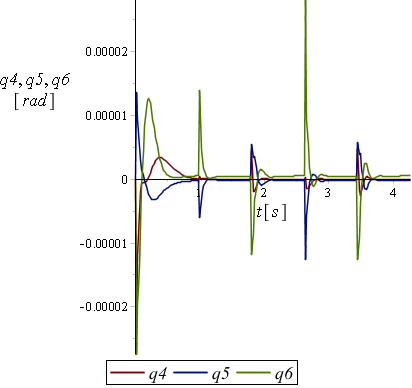
\includegraphics[width=\textwidth]{figs/t2_q456_base_testes}
        \caption{Rotações do ponto virtual}
        \label{fig::t2_q456_base_testes}
    \end{subfigure}
    \caption{Variações de posição e orientação da base de testes -- Tarefa 2}
    \label{fig::t2_q123456_base_testes}
\end{figure}

\begin{figure}[h!]
	\centering 
 	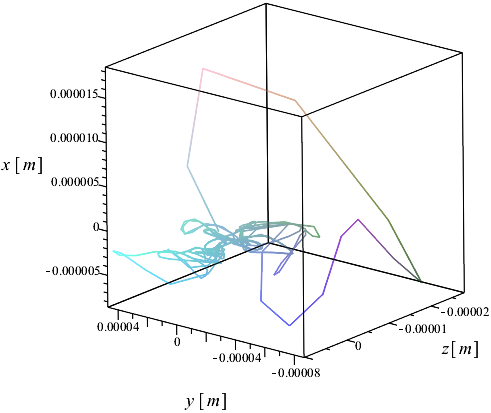
\includegraphics[width=0.70\textwidth]{figs/t2_pvirtural_base_testes}
 	\caption{Rastro da posição do ponto virtual -- Tarefa 2}
 	\label{fig::t2_pvirtural_base_testes}
\end{figure}


\subsubsection{Posição da ferramenta}

A Figura~\ref{fig::t2_posf_base_testes} fornece as posições efetiva e ideal da
Tarefa 2, e a Figura~\ref{fig::t2_erroposf_base_testes} o erro de cada
coordenada, com respeito ao referencial inercial.

\begin{figure}[h!]
	\centering 
 	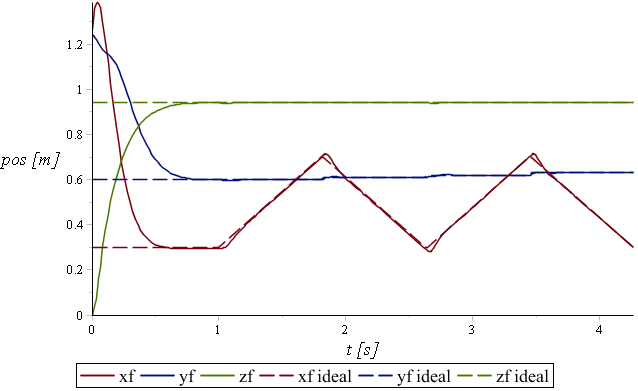
\includegraphics[width=0.75\textwidth]{figs/t2_posf_base_testes}
 	\caption{Posições das coordenadas da ferramenta para base de testes -- Tarefa
 	2}
 	\label{fig::t2_posf_base_testes}
\end{figure}

\begin{figure}[h!]
	\centering 
 	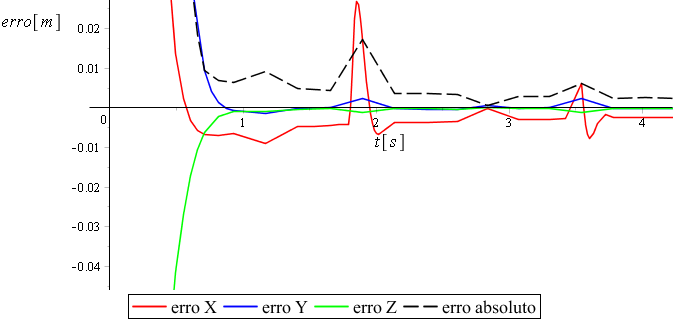
\includegraphics[width=0.75\textwidth]{figs/t2_erroposf_base_testes}
 	\caption{Erro de posição da ferramenta para base de testes -- Tarefa 2}
 	\label{fig::t2_erroposf_base_testes}
\end{figure}


\subsubsection{Velocidade da ferramenta}

A Figura~\ref{fig::t2_posf_base_testes} fornece as velocidades
efetivas e ideais . A Figura~\ref{fig::t2_erroposf_base_testes} o erro de cada
coordenada, com respeito ao referencial inercial.

\begin{figure}[h!]
	\centering 
 	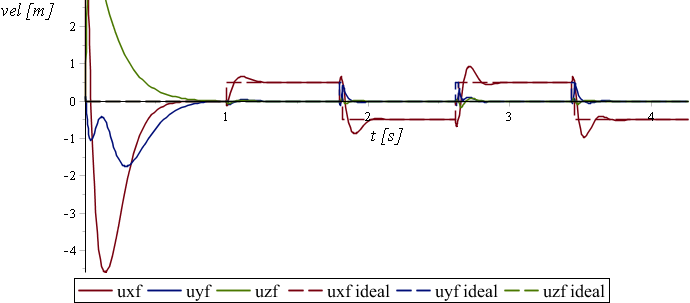
\includegraphics[width=0.75\textwidth]{figs/t2_velf_base_testes}
 	\caption{Velocidades das coordenadas da ferramenta base de testes --
 	Tarefa 2}
 	\label{fig::t2_velf_base_testes}
\end{figure}

\begin{figure}[h!]
	\centering 
 	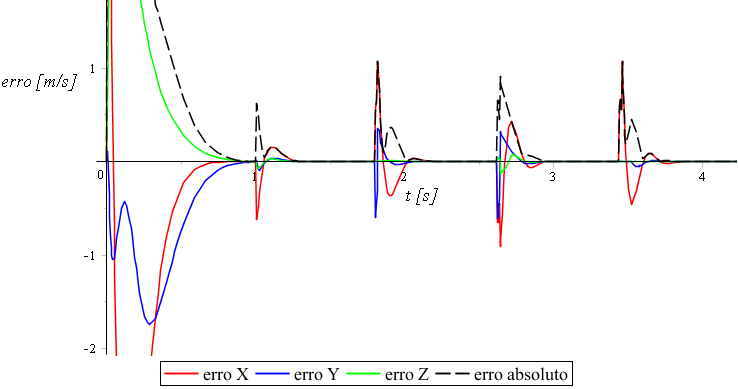
\includegraphics[width=0.75\textwidth]{figs/t2_errovelf_base_testes}
 	\caption{Erro de velocidade da ferramenta para base de testes --
 	Tarefa 2}
 	\label{fig::t2_errovelf_base_testes}
\end{figure}


\subsubsection{Orientação da ferramenta}

A Figura~\ref{fig::t2_erroori_base_testes} apresenta o erro de orientação da
ferramenta, representado pelo ângulo $\theta$.

\begin{figure}[h!]
	\centering 
 	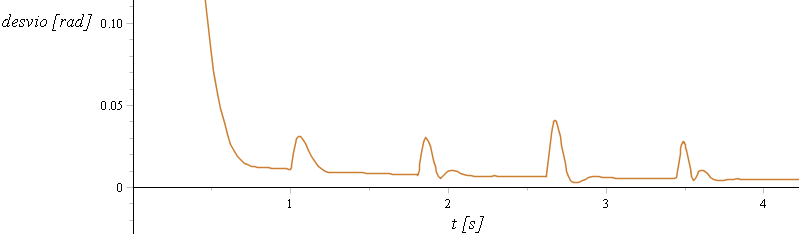
\includegraphics[width=0.75\textwidth]{figs/t2_erroori_base_testes}
 	\caption{Erro de orientação da ferramenta para base de testes -- Tarefa
 	2}
 	\label{fig::t2_erroori_base_testes}
\end{figure}


\subsection{Base PRP -- Tarefa 2}

\subsubsection{Posição do ponto virtual}

O reusltado da Figura~\ref{fig::t2_q123456_base_prp} apresenta a variação das
coordenadas generalizadas $q1$ a $q3$, referentes às translações, e $q4$ a $q6$,
referentes às rotações do ponto virtual de acoplamento base e robô. A
Figura~\ref{fig::t2_pvirtural_base_prp} ilustra o rastro da posição do ponto
virtual (origem do robô) no ambiente 3D.

\begin{figure}[h]
    \centering
    \begin{subfigure}[b]{0.48\textwidth}
        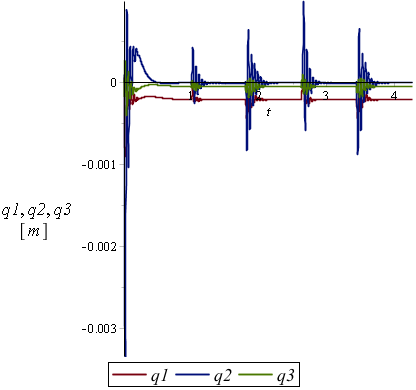
\includegraphics[width=\textwidth]{figs/t2_q123_base_prp}
        \caption{Deslocamentos do ponto virtual}
        \label{fig::t2_q123_base_prp}
    \end{subfigure}
    \quad %add desired spacing between images, e. g. ~, \quad, \qquad, \hfill
    % etc.
      %(or a blank line to force the subfigure onto a new line)
    \begin{subfigure}[b]{0.48\textwidth}
        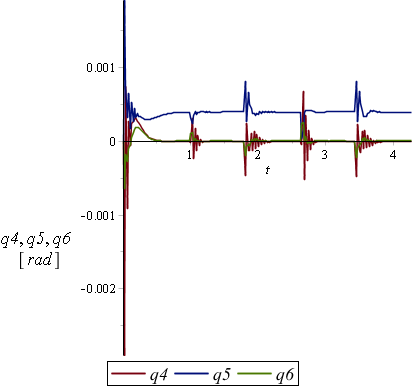
\includegraphics[width=\textwidth]{figs/t2_q456_base_prp}
        \caption{Rotações do ponto virtual}
        \label{fig::t2_q456_base_prp}
    \end{subfigure}
    \caption{Variações de posição e orientação da base PRP -- Tarefa 2}
    \label{fig::t2_q123456_base_prp}
\end{figure}

\begin{figure}[h!]
	\centering 
 	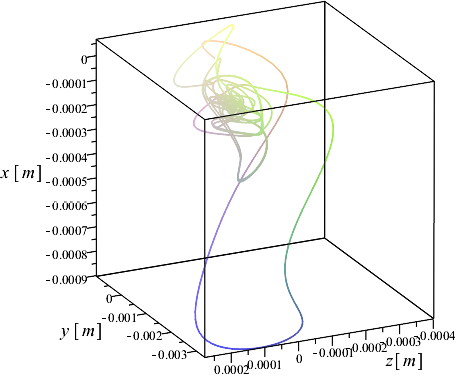
\includegraphics[width=0.70\textwidth]{figs/t2_pvirtural_base_prp}
 	\caption{Rastro da posição do ponto virtual -- Tarefa 2}
 	\label{fig::t2_pvirtural_base_prp}
\end{figure}


\subsubsection{Posição da ferramenta}

A Figura~\ref{fig::t2_posf_base_prp} fornece as posições efetiva e ideal da
Tarefa 2, e a Figura~\ref{fig::t2_erroposf_base_prp} o erro de cada
coordenada, com respeito ao referencial inercial.

\begin{figure}[h!]
	\centering 
 	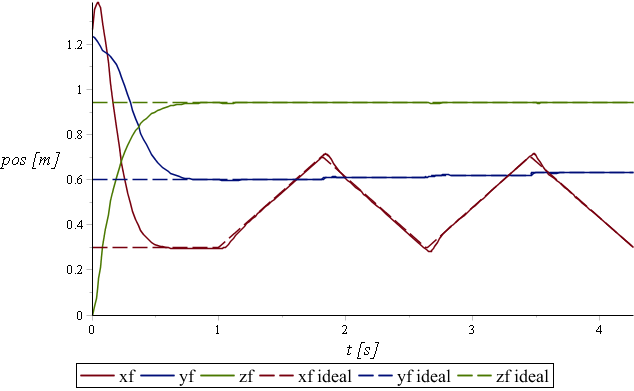
\includegraphics[width=0.75\textwidth]{figs/t2_posf_base_prp}
 	\caption{Posições das coordenadas da ferramenta para base PRP -- Tarefa
 	2}
 	\label{fig::t2_posf_base_prp}
\end{figure}

\begin{figure}[h!]
	\centering 
 	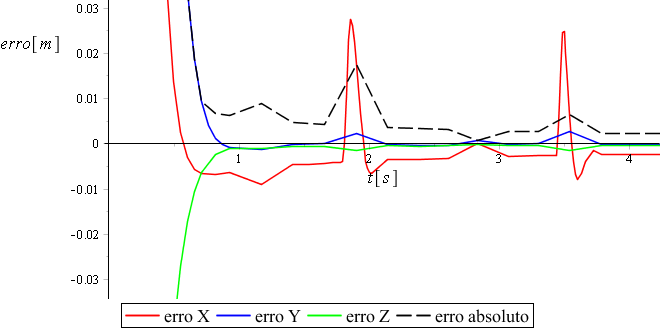
\includegraphics[width=0.75\textwidth]{figs/t2_erroposf_base_prp}
 	\caption{Erro de posição da ferramenta para base PRP -- Tarefa 2}
 	\label{fig::t2_erroposf_base_prp}
\end{figure}


\subsubsection{Velocidade da ferramenta}

A Figura~\ref{fig::t2_posf_base_prp} fornece as velocidades
efetivas e ideais . A Figura~\ref{fig::t2_erroposf_base_prp} o erro de cada
coordenada, com respeito ao referencial inercial.

\begin{figure}[h!]
	\centering 
 	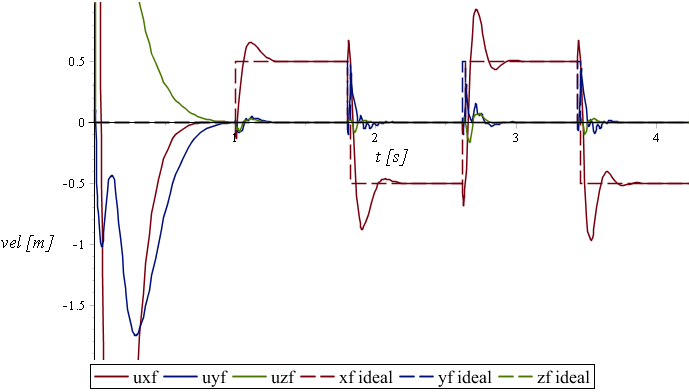
\includegraphics[width=0.75\textwidth]{figs/t2_velf_base_prp}
 	\caption{Velocidades das coordenadas da ferramenta base PRP --
 	Tarefa 2}
 	\label{fig::t2_velf_base_prp}
\end{figure}

\begin{figure}[h!]
	\centering 
 	\includegraphics[width=0.75\textwidth]{figs/t2_errovelf_base_prp}
 	\caption{Erro de velocidade da ferramenta para base PRP --
 	Tarefa 2}
 	\label{fig::t2_errovelf_base_prp}
\end{figure}


\subsubsection{Orientação da ferramenta}

A Figura~\ref{fig::t2_erroori_base_prp} apresenta o erro de orientação da
ferramenta, representado pelo ângulo $\theta$.

\begin{figure}[h!]
	\centering 
 	\includegraphics[width=0.75\textwidth]{figs/t2_erroori_base_prp}
 	\caption{Erro de orientação da ferramenta para base PRP -- Tarefa
 	2}
 	\label{fig::t2_erroori_base_prp}
\end{figure}


\clearpage
\subsection{Base PRPP -- Tarefa 2}

presenta-se os resultados das trajetórias considerando o manipulador montado
sobre a base modular PRP, da seção~\ref{sec::base_prpp}, realizando a Tarefa 2.

\subsubsection{Posição do ponto virtual}

O reusltado da Figura~\ref{fig::t2_q123456_base_prpp} apresenta a variação das
coordenadas generalizadas $q1$ a $q3$, referentes às translações, e $q4$ a $q6$,
referentes às rotações do ponto virtual de acoplamento base e robô. A
Figura~\ref{fig::t2_pvirtural_base_prpp} ilustra o rastro da posição do ponto
virtual (origem do robô) no ambiente 3D.

\begin{figure}[h]
    \centering
    \begin{subfigure}[b]{0.48\textwidth}
        \includegraphics[width=\textwidth]{figs/t2_q123_base_prpp}
        \caption{Deslocamentos do ponto virtual}
        \label{fig::t2_q123_base_prpp}
    \end{subfigure}
    \quad %add desired spacing between images, e. g. ~, \quad, \qquad, \hfill
    % etc.
      %(or a blank line to force the subfigure onto a new line)
    \begin{subfigure}[b]{0.48\textwidth}
        \includegraphics[width=\textwidth]{figs/t2_q456_base_prpp}
        \caption{Rotações do ponto virtual}
        \label{fig::t2_q456_base_prpp}
    \end{subfigure}
    \caption{Variações de posição e orientação da base PRPP -- Tarefa 2}
    \label{fig::t2_q123456_base_prpp}
\end{figure}

\begin{figure}[h!]
	\centering 
 	\includegraphics[width=0.64\textwidth]{figs/t2_pvirtural_base_prpp}
 	\caption{Rastro da posição do ponto virtual da base PRPP -- Tarefa 2}
 	\label{fig::t2_pvirtural_base_prpp}
\end{figure}

\subsubsection{Posição da ferramenta}

A Figura~\ref{fig::t2_posf_base_prpp} fornece as posições efetiva (linhas cheias)
e ideal (linhas tracejadas). E a Figura~\ref{fig::t2_erroposf_base_prpp} o erro
de cada coordenada, com respeito ao referencial inercial.

\begin{figure}[h!]
	\centering 
 	\includegraphics[width=0.75\textwidth]{figs/t2_posf_base_prpp}
 	\caption{Posições das coordenadas da ferramenta para base PRPP -- Tarefa
 	2}
 	\label{fig::t2_posf_base_prpp}
\end{figure}

\begin{figure}[h!]
	\centering 
 	\includegraphics[width=0.75\textwidth]{figs/t2_erroposf_base_prpp}
 	\caption{Erro de posição da ferramenta para base PRPP -- Tarefa 2}
 	\label{fig::t2_erroposf_base_prpp}
\end{figure}

\subsubsection{Velocidade da ferramenta}

São apresentados os gráficos da velocidade da ponta da ferramenta (linhas
cheias) e as velocidades de referência dadas pela cinemática inversa (linhas
tracejadas), na Figura~\ref{fig::t2_velf_base_prpp} e na
Figura~\ref{fig::t2_errovelf_base_prpp} os erros em relação a velocidade de
referência, no referencial inercial.

\begin{figure}[h!]
	\centering 
 	\includegraphics[width=0.75\textwidth]{figs/t2_velf_base_prpp}
 	\caption{Velocidades das coordenadas da ferramenta base PRPP --
 	Tarefa 2}
 	\label{fig::t2_velf_base_prpp}
\end{figure}

\begin{figure}[h!]
	\centering 
 	\includegraphics[width=0.75\textwidth]{figs/t2_errovelf_base_prpp}
 	\caption{Erro de velocidade da ferramenta para base PRPP --
 	Tarefa 2}
 	\label{fig::t2_errovelf_base_prpp}
\end{figure}

\subsubsection{Orientação da ferramenta}

A Figura~\ref{fig::t2_erroori_base_prpp} apresenta o erro de orientação,
representado pelo ângulo $\theta$.

\begin{figure}[h!]
	\centering 
 	\includegraphics[width=0.75\textwidth]{figs/t2_erroori_base_prpp}
 	\caption{Erro de orientação da ferramenta para base PRPP -- Tarefa
 	2}
 	\label{fig::t2_erroori_base_prpp}
\end{figure}

% -.~.-.~.-.~.-.~.-.~.-.~.-.~.-.~.-.~.-.~.-.~.-
\clearpage
\section{Comparação dos resultados} \label{sec::comparacao}

\subsection{Trajetórias}

A Figura~\ref{fig::res_traj1} apresenta a projeção no plano $xz$ da trajetória
da ferramenta (linha cheia) e a trajetória de referência (linha tracejada), para
realizar a Tarefa 1.

\begin{figure}[h]
    \centering
    \begin{subfigure}[b]{0.48\textwidth}
        \includegraphics[width=\textwidth]{figs/t1_traj_base_rig}
        \caption{Base rígida}
        \label{fig::t1_traj_base_rig}
    \end{subfigure}
    \quad %add desired spacing between images, e. g. ~, \quad, \qquad, \hfill
    % etc.
      %(or a blank line to force the subfigure onto a new line)
    \begin{subfigure}[b]{0.48\textwidth}
        \includegraphics[width=\textwidth]{figs/t1_traj_base_testes}
        \caption{Base de testes}
        \label{fig::t1_traj_base_testes}
    \end{subfigure}
    \quad %add desired spacing between images, e. g. ~, \quad, \qquad, \hfill
    % etc.
      %(or a blank line to force the subfigure onto a new line)
    \begin{subfigure}[b]{0.48\textwidth}
        \includegraphics[width=\textwidth]{figs/t1_traj_base_prp}
        \caption{Base PRP}
        \label{fig::t1_traj_base_prp}
    \end{subfigure}
    \quad %add desired spacing between images, e. g. ~, \quad, \qquad, \hfill
    % etc.
      %(or a blank line to force the subfigure onto a new line)
    \begin{subfigure}[b]{0.48\textwidth}
        \includegraphics[width=\textwidth]{figs/t1_traj_base_prpp}
        \caption{Base PRPP}
        \label{fig::t1_traj_base_prpp}
    \end{subfigure}
    \caption{Trajetórias da Tarefa 1 projetadas no plano $xz$ para cada base}
    \label{fig::res_traj1}
\end{figure}

A Figura~\ref{fig::res_traj2} apresenta a projeção no plano $xz$ da trajetória
da ferramenta (linha cheia) e a trajetória de referência (linha tracejada), para
realizar a Tarefa 1.

\begin{figure}[h]
    \centering
    \begin{subfigure}[b]{0.48\textwidth}
        \includegraphics[width=\textwidth]{figs/t2_traj_base_rig}
        \caption{Base rígida}
        \label{fig::t2_traj_base_rig}
    \end{subfigure}
    \quad %add desired spacing between images, e. g. ~, \quad, \qquad, \hfill
    % etc.
      %(or a blank line to force the subfigure onto a new line)
    \begin{subfigure}[b]{0.48\textwidth}
        \includegraphics[width=\textwidth]{figs/t2_traj_base_testes}
        \caption{Base de testes}
        \label{fig::t2_traj_base_testes}
    \end{subfigure}
    \quad %add desired spacing between images, e. g. ~, \quad, \qquad, \hfill
    % etc.
      %(or a blank line to force the subfigure onto a new line)
    \begin{subfigure}[b]{0.48\textwidth}
        \includegraphics[width=\textwidth]{figs/t2_traj_base_prp}
        \caption{Base PRP}
        \label{fig::t2_traj_base_prp}
    \end{subfigure}
    \quad %add desired spacing between images, e. g. ~, \quad, \qquad, \hfill
    % etc.
      %(or a blank line to force the subfigure onto a new line)
    \begin{subfigure}[b]{0.48\textwidth}
        \includegraphics[width=\textwidth]{figs/t2_traj_base_prpp}
        \caption{Base PRPP}
        \label{fig::t2_traj_base_prpp}
    \end{subfigure}
    \caption{Trajetórias da Tarefa 1 projetadas no plano $xy$ para cada base}
    \label{fig::res_traj2}
\end{figure}


\subsection{Erros máximos}

As Tabelas~\ref{tab::erros_t1} a \ref{tab::erros_t2} resumem os
erros máximos de posição, velocidade e orientação encontrados em cada tarefa. Os
erros de posição são dados nas 3 coordenadas cartesianas do referencial
inercial; o erro de velocidade é fornecido na direção tangente ao plano da
trajetória; e o erro de orientação é dado como um ângulo $\theta$ na direção do eixo $\omega$.

\begin{table}[h!]
\centering
\caption{Resumo dos erros máximos de cada base para Tarefa 1}
\label{tab::erros_t1}
\begin{tabular}{@{}lcccccc@{}}
\toprule
       & \multicolumn{3}{c}{\textbf{Posição $[mm]$}} & \textbf{Velocidade $[m/s]$} & \multicolumn{2}{c}{\textbf{Orientação $[rad]$}} 	\\ \midrule
         & x          & y          & z          & tangente            & $\theta$            & $\boldsymbol{\omega}$    		\\
Rígida & 1,5      	  & 9,0        & 20,0       & 0,30                &	0,021				& [0,995,~-0,960,~-0,029]		\\
Testes & 1,5    	  & 9,1        & 13,3       & 0,90                &	0,021				& [0.989,~-0,098,~0,111]		\\
PRP    & 8,0	 	  &	26,4	   & 8,6		& 0,70				  &	0,026				& [0,932,~-0,202,~0,301]						\\
PRPP   & 14,6  	 	  &	38,5	   & 12,9		& 0,98				  &	0,028				& [0,689,~-0,656,~0,308]		\\ \bottomrule
\end{tabular}
\end{table}


\begin{table}[h!]
\centering
\caption{Resumo dos erros máximos de cada base para Tarefa 2}
\label{tab::erros_t2}
\begin{tabular}{@{}lcccccc@{}}
\toprule
       & \multicolumn{3}{c}{\textbf{Posição $[mm]$}} & \textbf{Velocidade $[m/s]$} & \multicolumn{2}{c}{\textbf{Orientação $[rad]$}} 	\\ \midrule
         & x          & y          & z          & tangente            & $\theta$            & $\boldsymbol{\omega}$    		\\
Rígida & 0,07       & 16,5	   	& 11,5       	& 0,45                & 0,032				& [0,999,~0,002,~0,046] 		\\
Testes & 26,0     	& 2,2 	   	& 1,1			& 0,9                 & 0,041				& [-0,130,~-0.830,~0,557]		\\
PRP    & 27,4		& 2,6		& 1,5			& 0,44				  &	0,040				& [-0,043,~-0,826,~0,561]		\\
PRPP   & 31,8		& 32,2		& 15,0			& 1,09				  &	0,050				& [-0,083,~-0,798,~0,597]						\\ \bottomrule
\end{tabular}
\end{table}




% -.~.-.~.-.~.-.~.-.~.-.~.-.~.-.~.-.~.-.~.-.~.-
\section{Possíveis soluções} \label{sec::solucoes}

Apesar de o modelo de base rígida não ter apresentado uma trajetória perfeita, o
resultado aproximou-se da trajetória de referência, mantendo os erros aceitáveis
para as tarefas propostas. Dado que este modelo considera o robô sobre uma base
perfeitamente rígida, não ocorrem erros de trajetória devido a efeitos externos,
logo, as diferenças entre a trajetória de referência e a efetiva restringem-se,
pode-se dizer, às limitações do método de controle e devido ao torque entregue
pelos motores.

A presente pesquisa não tem o objetivo de comparar e estudar métodos de controle
para o manipulador robótico, tampouco alterar o projeto de manipuladores
industriais para ofereer melhor relação de torque e inércia. Lembra-se que esta
pesquisa visa oferecer ferramentas para prever a falha do sistema robô-base
flexível em realizar uma tarefa. Logo, a discussão de possíveis soluções
limita-se ao que diz respeito ao sistema acoplado. 

O método proposto tem a característica de possibilitar iterações no cenário
virtual de simulações. Isto propicia a verificação do projeto básico da
estrutura que propõe-se como base para o manipulador, quanto aos erros devido a
seu comportamento dinâmico. Logo, pode-se realizar modificações estruturais,
como alteração de geometria, materiais, espessura de perfis, contravetamentos,
reforços localizados, etc., que alteram as propriedades dinâmicas da base e
fornecem um novo resultado. O resultado é avaliado e comparado com os requisitos
do processo relacionado à tarefa e então aceito ou rejeitado. Se rejeitado,
pode-se realizar novas modificações, até convergir para um resultado que atende
às especificações; se aceito, pode-se pensar em uma otimização da estrutura de
base, visando minimizar a massa, o volume, o custo, ou qualquer outra
característica.

Comparando-se os resultados apresentados para a Tarefa 1, pela
Figura~\ref{fig::res_traj1}, conclui-se que para as bases de testes e modular
PRP houve um erro sistemático de defasagem, na direção $x$ da trajetória. Isto
pode ser explicado devido à posição de equilbrio estático do sistema acoplado
fornecer um erro de posição e de orientação da ferramenta do robô. Isto ocorre
porque quando o robô é montado sobre a base, esta se deforma até a posição de
equilíbrio estático. Se esta deformação não é considerada, resulta no erro
sistemático apresentado nas duas versões de base. Interessanetemente, este erro
não é tão acentuado para a Tarefa 2, como pode ser verificado na
Figura~\ref{fig::res_traj2}.

Uma solução para este erro estático seria o reforço estrutural da base contra as
deformações que resultam o erro nesta direção. Uma opção com o mínimo de impacto
no projeto original seria o acréscimo de contraventamentos, ou braços de apoio,
a partir da estrura até a superfície do ambiente, como pode ser verificado na
Figura~\ref{fig::contraventamentos}

\begin{figure}[h!]
	\centering 
 	\includegraphics[width=0.55\textwidth]{figs/contraventamentos}
 	\caption{Reforços estruturais para estrutura da base modular PRP}
 	\label{fig::contraventamentos}
\end{figure}

Não garante-se que esta modificação irá solucionar o problema, por isso, deve-se
realizar uma iteração do método. Para esta solução, deve-se incluir os reforços
estruturais no modelo AEF da base, obter-se daí uma nova matriz de rigidez, e
então simular o novo sistema.

Outra solução contra os erros sistemáticos devido à deformação estática da base
é a calibração da posição resultante do robô após instalação. No projeto EMMA,
esta calibração é realizada por meio de escaneamento 3D, que gera uma nuvem de
pontos que permite a identificação e localização do robô e do ambiente.
Identificando-se a pose inicial do robô, em relação a um referencial, pode-se
calibrar a nova pose e eliminar tais erros sistemáticos. Porém, esta solução não
elimina erros dinâmicos porque a calibração é realizada antes da operação,
estaticamente.

Verifica-se em todos os resultados que quando há variação da direção da
trajetória os erros de posição, velocidade e orientação aumentam abruptamente.
Logo, nas regiões próximas às extermidades dos paralelos, os requisitos do
processo de revestimento não são atendidos. Uma solução neste caso é a
utilização de placas de sacrifício, que se sobrepõem ao material base a ser
revestido e garantem que a faixa exposta ao revestimento esteja com os
requisitos dentro de uma tolerância aceitável. Logo, estas placas devem ser
posicionadas a cobrir a região onde ocorrem os erros mais acentuados, nas
extremidades dos paralelos, conforme demonstrado na
Figura~\ref{fig::sacrificio}.

\begin{figure}[h!]
	\centering 
 	\includegraphics[width=0.80\textwidth]{figs/sacrificio}
 	\caption{Placas de sacrifício para delimitar faixa aceitável}
 	\label{fig::sacrificio}
\end{figure}

Pelo o resultado da base telescópica PRPP, Figuras~\ref{fig::res_traj1} e
\ref{fig::res_traj2}, percebe-se claramente que o sistema acoplado falhou em
realizar as tarefas, dados os grandes erros de trajetória. Os resultados de
posição e orientação do referencial localizado no ponto virtual da base, dados
pelas Figuras~\ref{fig::t1_pvirtural_base_prpp} e
\ref{fig::t2_pvirtural_base_prpp} demonstram grandes oscilações, da ordem de
$20~mm$ e $0,04~rad$ de amplitude. Estas oscilações propagadas até a ponta da
ferramenta resultam nos erros de trajetória apresentados. Esta base telescópica
utilizada com o robô MH12 demonstrou-se muito flexível e inviável para a
aplicação.

O controle do sistema acoplado atua apenas nas juntas do robô. No entanto, se
temos conhecimento suficiente da dinâmica do sistema, que inclui os movimentos
dinâmicos da base, pode-se desenvolver métodos de controle para compensar estes
movimentos. \citet{lew2001simple} propõem um método de controle cujo objetivo é
determinar o torque de entrada das juntas do manipulador, de forma que as
oscilações da base $q1$ a $q6$ amorteçam o mais rapidamente possível, enquanto
os ângulos de juntas do robô $q7$ a $q11$ seguem o caminho desejado. O algoritmo
de controle utiliza o \textit{feedback} dos sensores de oscilação da base para
modular as entradas dos atuadores e induzir forças de inércia dissipativas.

Lembra-se que a análise modal experimental da base foi possível graças à
instrumentação da base por acelerômetros. Os acelerômetros foram distribuidos e
seus dados processados de forma que se obtivesse a aceleração em cada grau de
liberdade no ponto virtual da base. Estas acelerações, se integradas, fornecem
justamente as coordenadas generalizadas $q1$ a $q6$ ou as velocidades
generalizadas $u1$ a $u6$. Logo, pode-se incluir estes parâmetros nas
estratégias de controle do robô, a fim de minimizar as oscilações da base.
Existem diversas outras estratégias (\cite{george2002inertial},
\cite{kwon1994input}, \cite{tahboub1998intelligent} e
\cite{nenchev1999reaction}) que atuam no controle das juntas do manipulador,
dado o conhecimento da dinâmica da base e estas podem ser exploradas nos modelos
construídos neste trabalho.


% if we have a proper knowledge about the dynamics of the system including the
% base motion dynamics, we can develop sophisticated control methods.
% (Artigo: Moving base robotics and reaction management control)
